\documentclass[
    10pt,
    aspectratio=169,
]{beamer}
\usepackage{transparent}
\usepackage{booktabs} 
\usepackage{tabularx}
\usepackage{makecell}
\beamertemplatenavigationsymbolsempty
%\usepackage{appendixnumberbeamer} %If you want a separate slide counter for your appendix
\usepackage{tikz}
\usepackage{colortbl}
%%% To add citations
\usepackage[
    style=nature,
    sorting=none,
    isbn=false,
    url=false,
    doi=true,
    eprint=false,
    date=year,
    maxnames=3,
    minnames=2
]{biblatex}
\addbibresource{bibliography.bib}
\renewcommand*{\bibfont}{\normalfont\fontsize{5}{5}\selectfont}
\usepackage{algorithm}
\usepackage{algpseudocode}
\usepackage{lipsum}
\usepackage{hyperref}
%%% Customize Theme %%%%%%%%%%%%%%%%%%%%%%
\usetheme[width=3.8em]{boxes} %Beamer themes here https://deic.uab.cat/~iblanes/beamer_gallery/index_by_theme.html


% \addtobeamertemplate{sidebar right}{}{ 
%  \hspace*{.5em}{\transparent{0.5} \includegraphics[width = 0.131\textwidth]{University_of_Southern_California_seal.svg.png}}%
% }

%----------------------------------------------------------
%           Colour Setup
%----------------------------------------------------------

%fg = font color
%bg = background color

% ! WARNING ! : Many colors are linked to multiple attributes, so changing one color can have unexpected changes!

% If you want to tweak the shading of orange and red, tweak the below 2 lines:
\definecolor{myRed}{RGB}{153, 0, 0}
\definecolor{myOrange}{RGB}{255, 204, 0}
\definecolor{tableGreen}{RGB}{144, 238, 144}
\definecolor{tableOrange}{RGB}{255, 204, 0}

\setbeamertemplate{sidebar canvas right}[vertical shading][top=myRed, middle=myRed!85, bottom=myRed]
% Bottom right hand color
\setbeamercolor*{structure}{bg=myOrange,fg=myRed}

\setbeamercolor*{palette primary}{use=structure,fg=white,bg=structure.fg} %?
\setbeamercolor*{palette secondary}{use=structure,fg=myRed,bg=myOrange}
    %bottom left of footer & bar between title & top bubbles
\setbeamercolor*{palette tertiary}{use=structure,fg=white,bg=myRed} 

\setbeamercolor{frametitle}{bg=myRed,fg=white} %title of each slide

\setbeamercolor*{titlelike}{parent=palette primary} %?



%%% Edits ONLY the TOC slide %%%
\setbeamercolor{section in toc}{fg=black}
\setbeamercolor{subsection in toc}{fg=black}

%%% Block Colors %%%
% Standard block %
    \setbeamercolor{block title}{bg=myOrange, fg=white}
    \setbeamercolor{block body}{bg=myOrange!20}

% Alerted block % If you want to customize it's color
    %\setbeamercolor{block title alerted}{bg=cyan, fg=white}
    %\setbeamercolor{block body alerted}{bg=cyan!10}

% Example block % If you want to customize it's color
    %\setbeamercolor{block title example}{bg=cyan, fg=white}
    %\setbeamercolor{block body example}{bg=cyan!10}

\setbeamercolor{title in sidebar}{fg=white!75}
\setbeamercolor{author in sidebar}{fg=white!50}
\setbeamercolor{palette sidebar secondary}{fg=myRed,bg=white!80}
\setbeamercolor{subsection in sidebar}{fg=myRed,bg=white!80}
\setbeamercolor{section in sidebar shaded}{fg=white!75}
\setbeamercolor{subsection in sidebar shaded}{fg=white!75}
%---------------------------------------------------------
%	SELECT FONT THEME & FONTS
%---------------------------------------------------------

\usefonttheme{serif}
\usepackage{fontenc}
\usepackage{ebgaramond}

\setbeamerfont{frametitle}{size=\large}

%---------------------------------------------------------
%	SELECT OUTER THEME
%---------------------------------------------------------
% Outer themes change the overall layout of slides, such as: header and footer lines, sidebars and slide titles. Uncomment each theme in turn to see what changes it makes to your presentation.

\useoutertheme{default}

% This sets up the footer on each slide

\setbeamercolor{section in foot}{fg=white, bg=myRed}


\setbeamertemplate{footline}
{
 \hbox{%
  \begin{beamercolorbox}[wd=.12\paperwidth,ht=2.6ex,dp=2ex,center]{section in foot}%
    \usebeamerfont{section in foot}\insertshortauthor
  \end{beamercolorbox}%
  
  \begin{beamercolorbox}[wd=.65\paperwidth,ht=2.6ex,dp=2ex,center]{section in foot}%
    \usebeamerfont{section in foot} ICD-10 Classification \hspace{1em} \insertframenumber/\inserttotalframenumber
  \end{beamercolorbox}%
  
  \begin{beamercolorbox}[wd=.2\paperwidth,ht=2.6ex,dp=2ex,center]{section in foot}%
    \usebeamerfont{section in foot} 
  \end{beamercolorbox}}%

  \vskip0pt%
}



% Other Frames to consider...

%\useoutertheme{miniframes}
%\useoutertheme{infolines}
%\useoutertheme{smoothbars}
%\useoutertheme{sidebar}
%\useoutertheme{split}
%\useoutertheme{shadow}
%\useoutertheme{tree}
%\useoutertheme{smoothtree}

%---------------------------------------------------------
%	PRESENTATION INFORMATION
%---------------------------------------------------------

\title[ICD-10 Classification]{ICD-10 Disease Classification Experiments}
%\subtitle{Subtitle Space}
\author[D. Best]{Darrell Best}

\date{\today}
\institute[ISI]{Information Sciences Institute \\ 
University of Southern California }

%%% This sets up the title page

\titlegraphic{
  \begin{tikzpicture}[remember picture, overlay]
    % 
    \node[anchor=south west, xshift=0cm, yshift=0.5cm] at (current page.south west) {
      
\includegraphics[height=1cm]{logos/USC_seal.png}
    };

    % 
    \node[anchor=south east, xshift=-0.5cm, yshift=0.5cm] at (current page.south east) {
      
\includegraphics[height=1cm]{logos/isi.png}
    };
    
    % % 
    % \node[anchor=north east, xshift=-0.8cm, yshift=-0.3cm] at (current page.north east) {
    %   \includegraphics[height=1.1cm]{logos/CleanEasy-logo3.png}
    % };
    
    % %
    % \node[anchor=north east, xshift=-2.8cm, yshift=-0.3cm] at (current page.north east) {
    %   \includegraphics[height=1.4cm]{logos/CleanEasy-logo4.png}
    % };
  \end{tikzpicture}
}
% \setbeamertemplate{title page}{
%   \begin{minipage}[b][\paperheight]{\textwidth}
%     \vfill%
%     \ifx\inserttitle\@empty\else\usebeamertemplate*{title}\fi
%     \ifx\insertsubtitle\@empty\else\usebeamertemplate*{subtitle}\fi
%     \usebeamertemplate*{title separator}
%     \ifx\beamer@shortauthor\@empty\else\usebeamertemplate*{author}\fi
%     \ifx\insertdate\@empty\else\usebeamertemplate*{date}\fi
%     \ifx\insertinstitute\@empty\else\usebeamertemplate*{institute}\fi
%     \vfill
%     \vspace*{1mm}
%   \end{minipage}
%     \raisebox{.1\paperheight}[1.7em][0em]{%
%     \makebox[\paperwidth][c]{%
%       \hspace*{-8.2em}\includegraphics[width=.883\paperwidth,height=1cm]{PHP.png}%
%     }%
%   }
% }
\makeatother

%---------------------------------------------------------
%---------------------------------------------------------
%---------------------------------------------------------
\begin{document}

%---------------------------------------------------------
%	TITLE SLIDE
%---------------------------------------------------------
\section{}
\begin{frame}
	\titlepage % Output the title slide, automatically created using the text entered 
\end{frame}

%---------------------------------------------------------
%	TABLE OF CONTENTS SLIDE
%---------------------------------------------------------
% References sections and subsections, specified with the standard \section and \subsection commands. If you want to display all sections and subsections on one slide, just use \tableofcontents. If you want to just display each section one at a time (in subsequent slides) use \tableofcontents[pausesections].

%\tableofcontents



%---------------------------------------------------------
%	PRESENTATION BODY SLIDES
%---------------------------------------------------------

%==========================================================
% SECTION 1: INTRODUCTION & METHODS
%==========================================================

% \section{Introduction}
\begin{frame}{Introduction}
\begin{itemize}
    \item This binary classification system serves as a first-pass filter to identify relevant documents before sending them into the full processing pipeline, reducing computational costs by filtering out irrelevant data early.
    \item It identifies whether text segments contain relevant symptomology phrasing that warrants further analysis in the main pipeline, allowing us to filter out documents that don't contain symptom-related content early and reduce processing costs.
    \item The labeled data Team 2 is working on focuses specifically on symptomology phrasing, which will serve as the positive class for our binary classification target.
    \item Similar techniques can be adapted on the full scope of ICD-10 codes for other needed areas.
\end{itemize}
\end{frame}

\begin{frame}{Dataset}
\begin{itemize}
    \item \textbf{Data Source:} MIMIC-IV clinical discharge summaries
    \begin{itemize}
        \item Free-text clinical narratives documenting patient hospital stays
        \item Contains detailed symptomology, diagnoses, and treatment information
        \item De-identified for privacy protection
    \end{itemize}
    \item \textbf{Target Condition:} Dementia diagnosis (ICD-10 code F03)
    \begin{itemize}
        \item Selected for sufficient sample size and clinical relevance
        \item Binary classification: presence vs. absence of F03 diagnosis
    \end{itemize}
    \item \textbf{Dataset Composition:}
    \begin{itemize}
        \item 7,286 total samples (3,643 positive, 3,643 negative)
        \item Negative samples randomly sampled from patients without F03 diagnosis
        \item Balanced dataset to prevent class bias
        \item Split: 70\% training (5,099), 20\% test (1,458), 10\% validation (729)
    \end{itemize}
    \item \textbf{Preprocessing:} Text cleaning, tokenization, stop-word removal
\end{itemize}
\end{frame}

\begin{frame}{Embeddings}
\begin{itemize}
    \item We extracted features from the text using the following embedding models:
    \begin{itemize}
        \item \textbf{TF-IDF} (5000 features) - Term frequency-inverse document frequency
        \item \textbf{Word2Vec} (300 features) - Word embeddings averaged to document level
        \item \textbf{Doc2Vec} (300 features) - Document-level paragraph vectors (PV-DM \& PV-DBOW)
        \item \textbf{FastText} (300 features) - Character n-gram aware embeddings
        \item \textbf{BioBERT} (768 features) - Biomedical domain BERT
        \item \textbf{SciBERT} (768 features) - Scientific text BERT
        \item \textbf{PubMedBERT} (768 features) - PubMed-trained BERT
    \end{itemize}
\end{itemize}
\end{frame}

\begin{frame}{Models Tested: 34 Total}
\small
\begin{columns}[t]
\column{0.5\textwidth}
\textbf{TF-IDF Based (14 models)}
\begin{itemize}
  \item \textbf{Boosting (4):} LightGBM, XGBoost, CatBoost, AdaBoost
  \item \textbf{Linear (2):} Logistic Regression, Linear SVM
  \item \textbf{Trees (3):} Random Forest, Extra Trees, Naive Bayes
  \item \textbf{Distance (4):} KNN, Radius Neighbors, Nearest Centroid, Cosine Similarity
  \item \textbf{Neural (1):} Neural Network
\end{itemize}

\column{0.5\textwidth}
\textbf{Embedding Based (20 models)}
\begin{itemize}
  \item \textbf{Word2Vec (5):}
  \begin{itemize}
    \scriptsize
    \item Logistic, LightGBM, XGBoost, CatBoost, AdaBoost
  \end{itemize}
  \item \textbf{Doc2Vec PV-DM (5):}
  \begin{itemize}
    \scriptsize
    \item Logistic, LightGBM, XGBoost, CatBoost, AdaBoost
  \end{itemize}
  \item \textbf{Doc2Vec PV-DBOW (5):}
  \begin{itemize}
    \scriptsize
    \item Logistic, LightGBM, XGBoost, CatBoost, AdaBoost
  \end{itemize}
  \item \textbf{FastText (5):}
  \begin{itemize}
    \scriptsize
    \item Logistic, LightGBM, XGBoost, CatBoost, AdaBoost
  \end{itemize}
\end{itemize}
\end{columns}
\end{frame}

%   \item \textbf{Notes:}
%     \begin{itemize}
%       \item \textsuperscript{*}Models marked with an asterisk are linear \emph{in the embedding space} if the encoder is frozen; end-to-end fine-tuning makes the overall system non-linear (the classification head remains linear).
%       \item AdaBoost is a boosting method (often with decision stumps) but not part of the gradient-boosted decision tree family.
%     \end{itemize}
% \end{itemize}

%==========================================================
% SECTION 2: RESULTS
%==========================================================

% \section{Model Performance}
\begin{frame}{Model Performance Summary}
\begin{itemize}
    \item We evaluated 34 models for binary classification (14 TF-IDF based, 20 advanced embeddings).
    \item The following table summarizes the model evaluation metrics for the ten best performing models.
\end{itemize}
\vspace{-0.19cm}
\begin{table}[]
\small
\begin{tabular}{|l|c|c|c|c|c|}
\hline
\textbf{}                       & \textbf{Accuracy}                                              & \textbf{Precision}                      & \textbf{Recall}                         & \textbf{F1}                             & \textbf{AUC}                                                   \\ \hline
\textbf{LightGBM}               & \cellcolor[HTML]{90EE90}{\color[HTML]{000000} \textbf{0.9540}} & \cellcolor[HTML]{FFD700}0.9572 & \cellcolor[HTML]{90EE90}{\color[HTML]{000000} \textbf{0.9506}} & \cellcolor[HTML]{90EE90}\textbf{0.9539} & \cellcolor[HTML]{90EE90}{\color[HTML]{000000} \textbf{0.9879}} \\ \hline
\textbf{XGBoost}                & \cellcolor[HTML]{FFD700}0.9520                                 & 0.9570                                  & 0.9465                                  & \cellcolor[HTML]{FFD700}0.9517          & 0.9862                                 \\ \hline
\textbf{CatBoost}               & 0.9458                                                         & \cellcolor[HTML]{90EE90}{\color[HTML]{000000} \textbf{0.9577}}                                  & 0.9328                                  & 0.9451                                  & \cellcolor[HTML]{FFD700}0.9865                                                         \\ \hline
\textbf{AdaBoost}               & 0.9355                                                         & 0.9416                                  & 0.9287                                  & 0.9351                                  & 0.9823                                                         \\ \hline
\textbf{Doc2Vec-LogisticPVDBOW} & 0.9328                                                         & 0.9201                                  & 0.9479 & 0.9338                                  & 0.9780                                                         \\ \hline
\textbf{Random Forest}          & 0.9259                                                         & 0.9080                                  & \cellcolor[HTML]{FFD700}0.9479 & 0.9275                                  & 0.9776                                                         \\ \hline
\textbf{Linear SVM}             & 0.9225                                                         & 0.9173                                  & 0.9287                                  & 0.9230                                  & 0.9745                                                         \\ \hline
\textbf{Logistic Regression}    & 0.9177                                                         & 0.9055                                  & 0.9328                                  & 0.9189                                  & 0.9722                                                         \\ \hline
\textbf{Extra Trees}            & 0.9088                                                         & 0.8901                                  & 0.9328                                  & 0.9109                                  & 0.9656                                                         \\ \hline
\textbf{Neural Network}         & 0.9060                                                         & 0.9044                                  & 0.9081                                  & 0.9062                                  & 0.9644                                                         \\ \hline
\end{tabular}
\end{table}

\fcolorbox{tableGreen}{tableGreen}{\rule{0pt}{6pt}\rule{6pt}{0pt}} \scriptsize 1st place
\fcolorbox{tableOrange}{tableOrange}{\rule{0pt}{6pt}\rule{6pt}{0pt}} \scriptsize 2nd place
% \scriptsize \cellcolor[HTML]{90EE90} = 1st place \quad \cellcolor[HTML]{FFD700} = 2nd place
\end{frame}

\begin{frame}{Model Comparison - All Metrics}
\begin{figure}
    \centering
    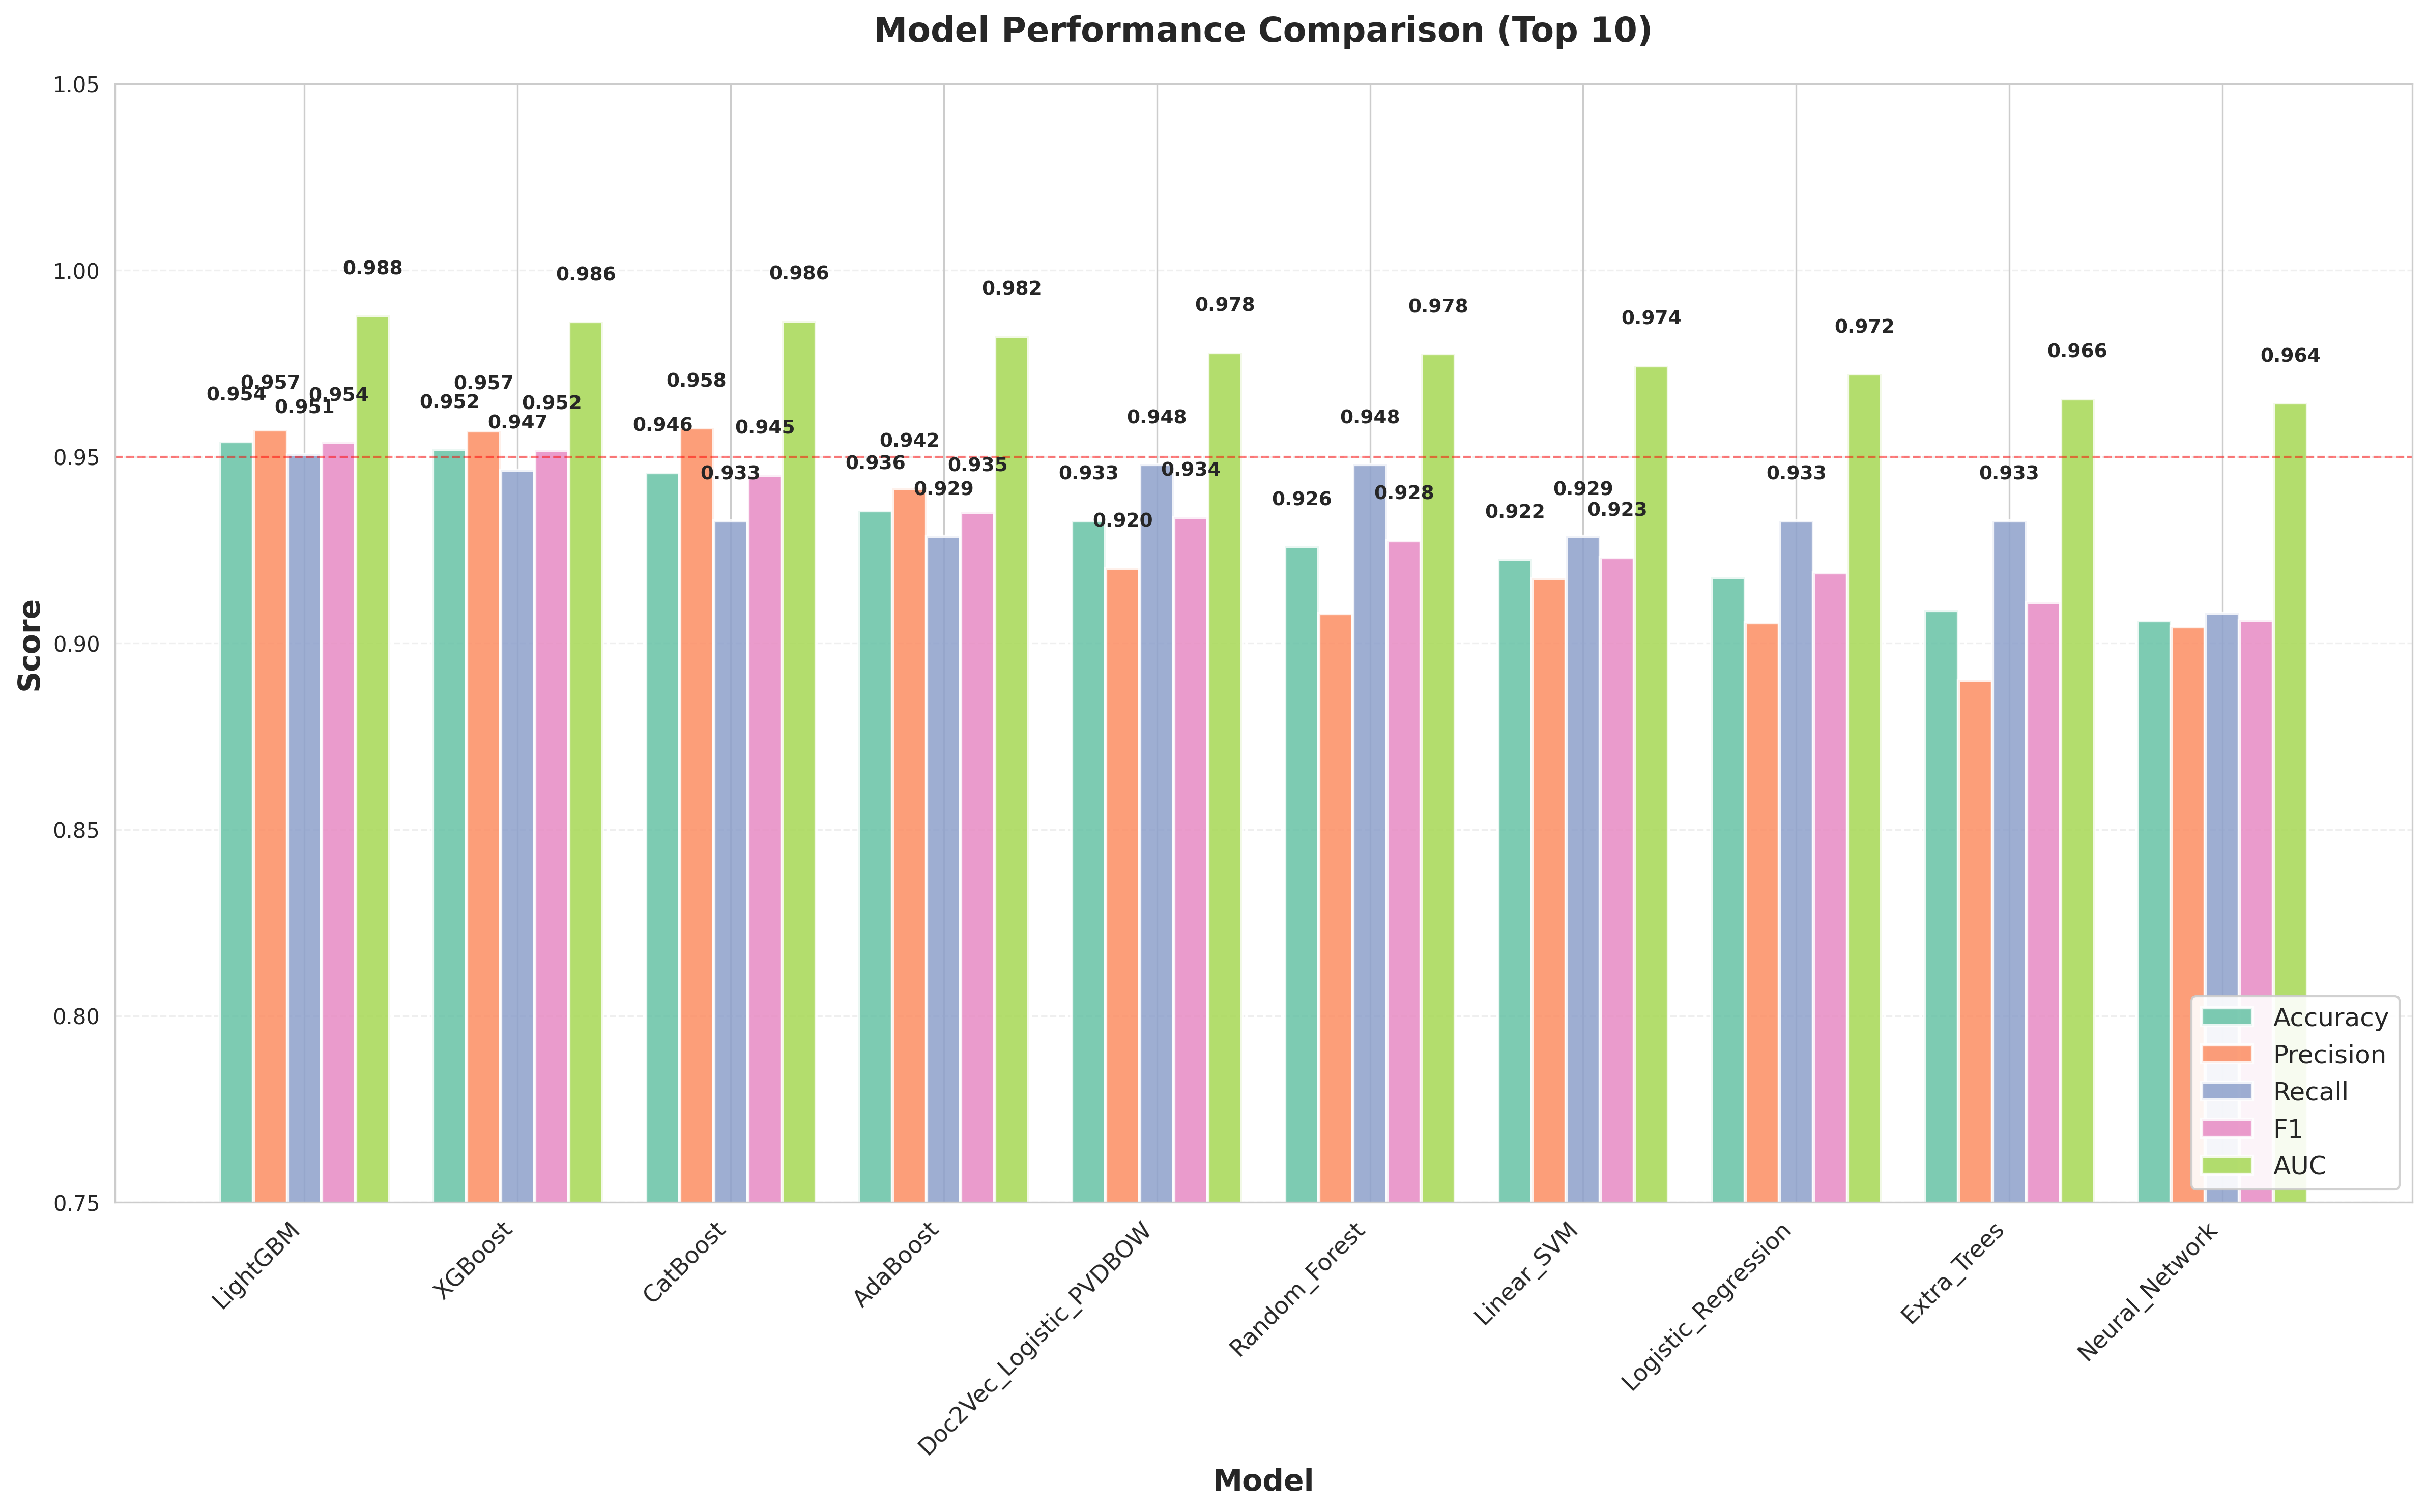
\includegraphics[width=0.85\linewidth]{experiment_figures/model_comparison.png}
    \label{fig:model_comparison}
\end{figure}
\end{frame}

\begin{frame}{ROC Curves}
\begin{figure}
    \centering
    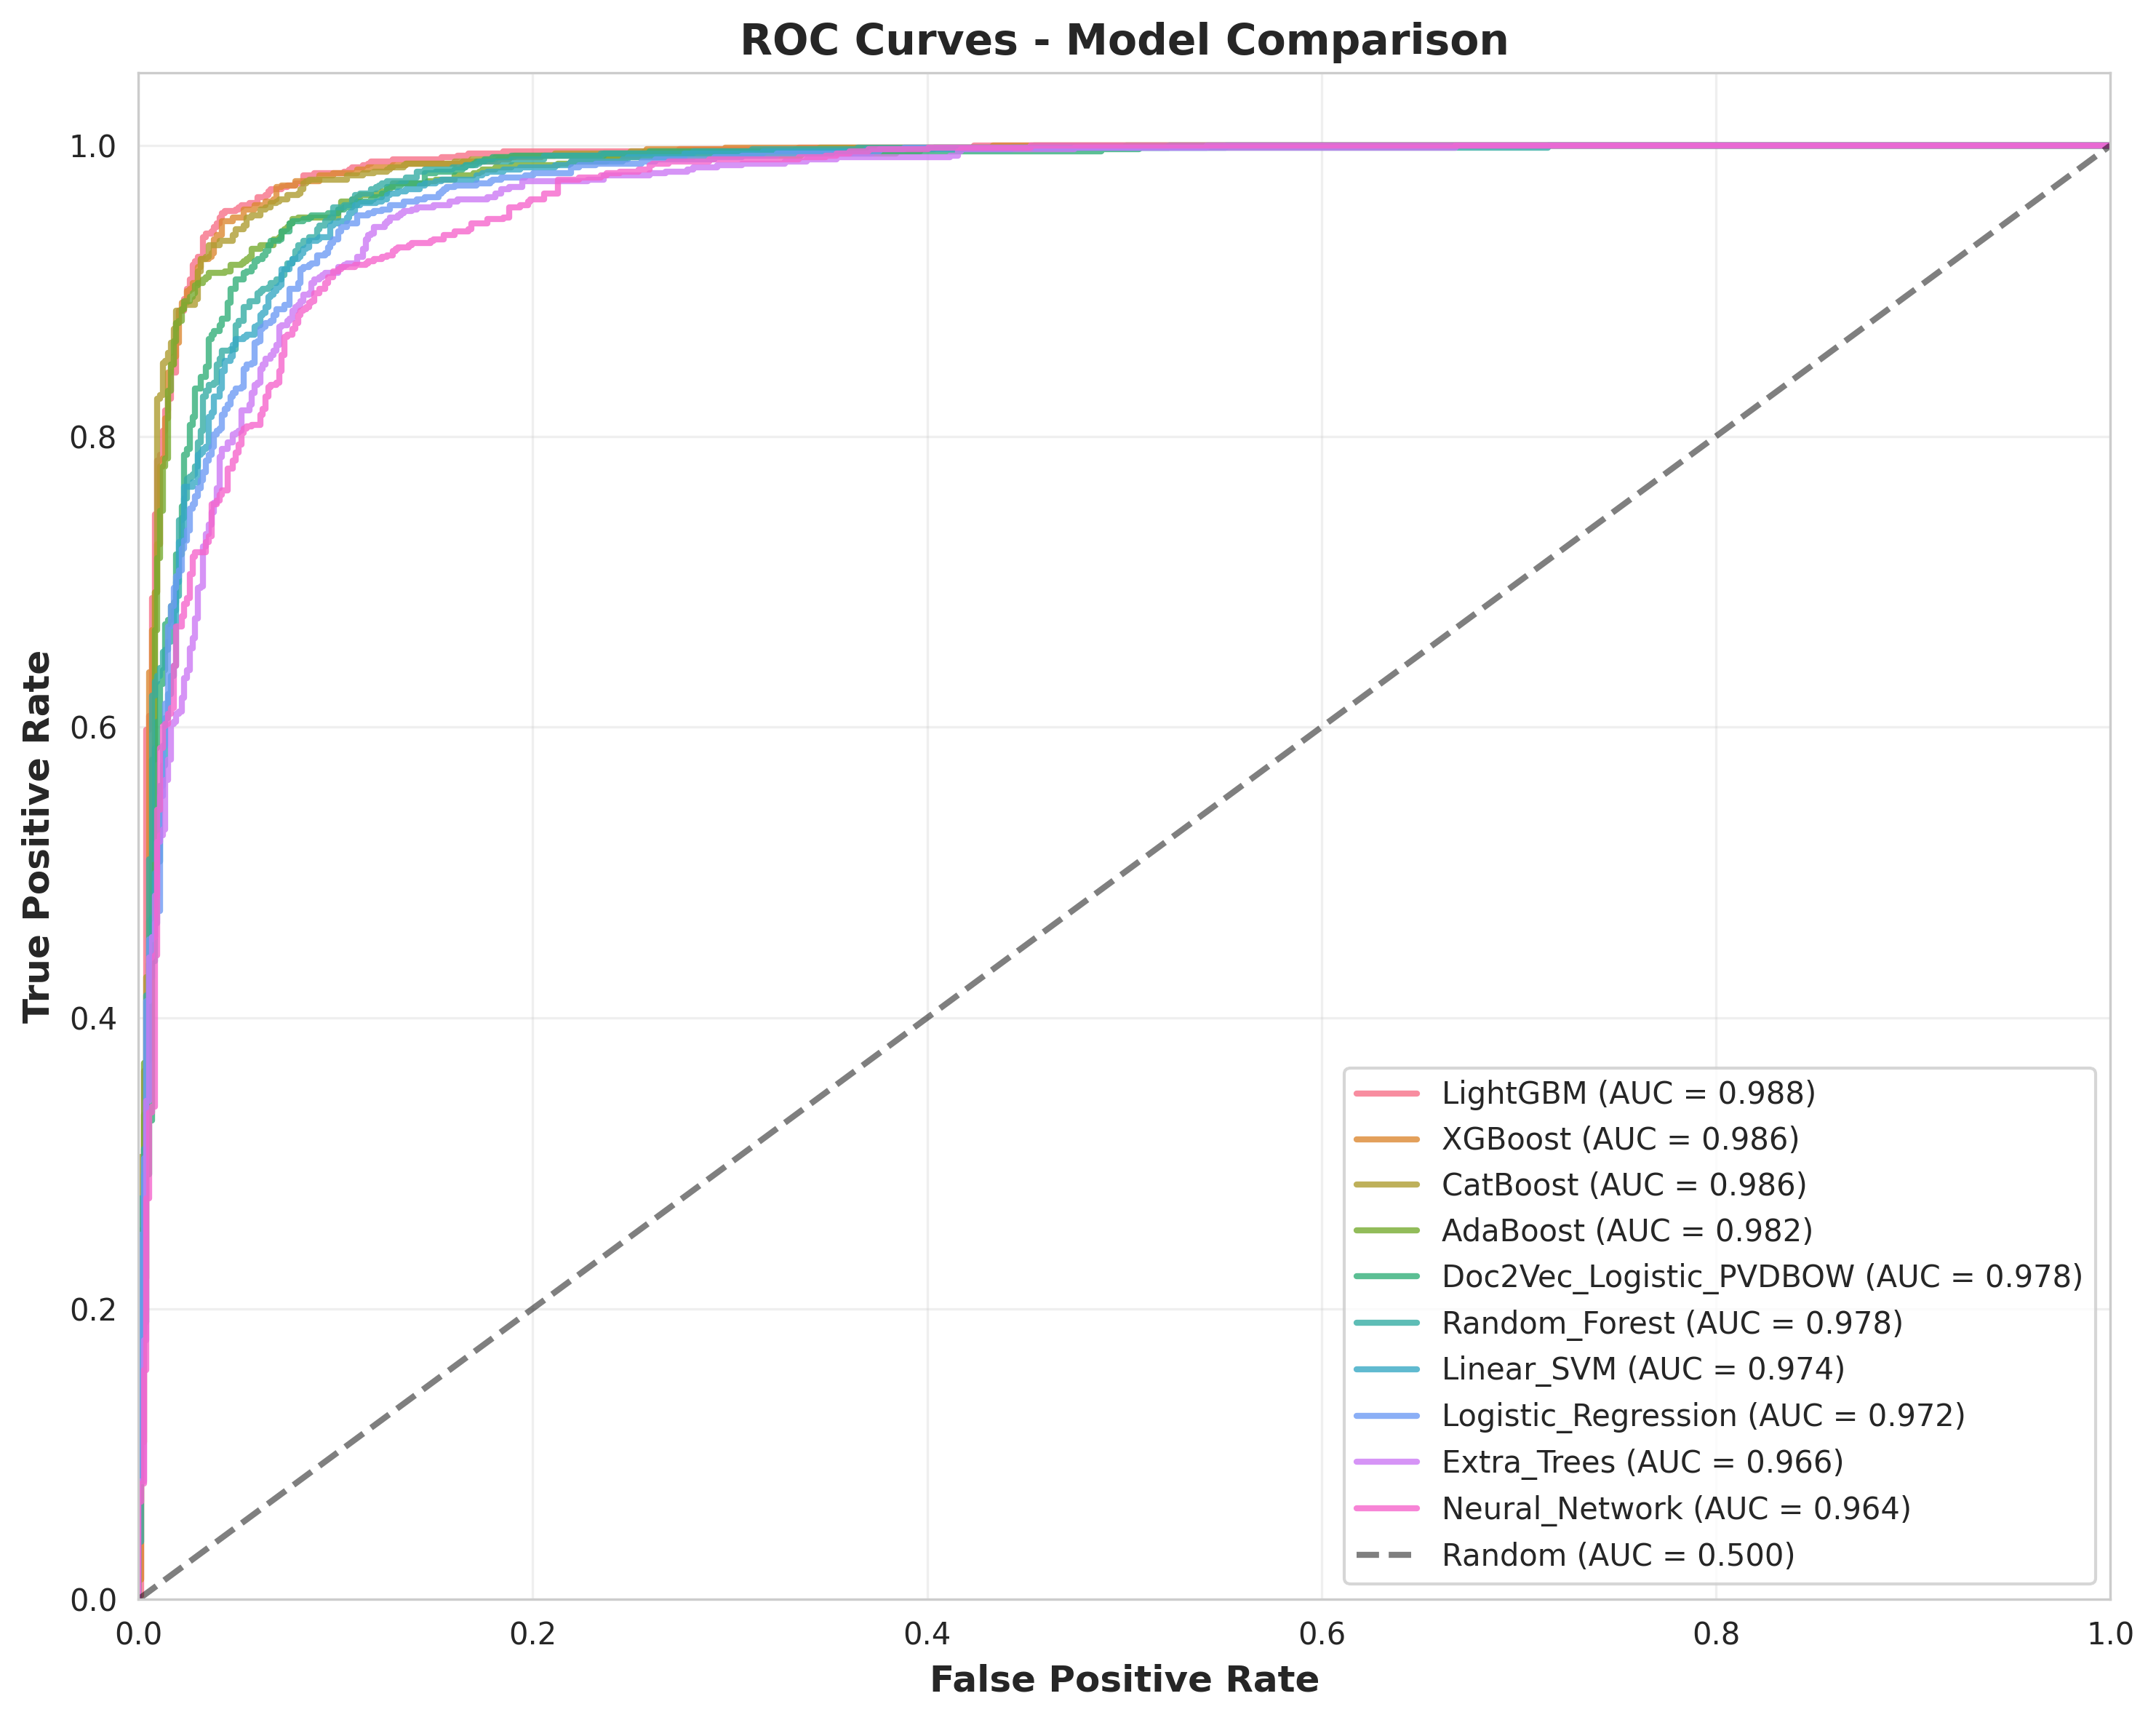
\includegraphics[width=0.65\linewidth]{experiment_figures/roc_curves.png}
    \label{fig:ROC}
\end{figure}
\end{frame}

\begin{frame}{Statistical Significance Tests}
\begin{itemize}
    \item Gradient boosting methods demonstrated clear superiority, with all four boosting variants achieving F1 scores between 93.5\% and 95.4\%.
    \item McNemar's statistical tests (45 pairwise comparisons on top 10 models) confirmed these models significantly outperform all other approaches.
    \item LightGBM and XGBoost showed no statistically significant difference ($p=0.25$), though LightGBM significantly outperformed CatBoost ($p=0.002$).
    \item All boosting models significantly outperformed linear models ($p < 0.001$).
\end{itemize}
\end{frame}

\begin{frame}{TF-IDF vs Embedding Models}
\begin{table}[]
\centering
\small
\begin{tabular}{|l|c|c|c|}
\hline
\textbf{Model} & \textbf{F1 Score} & \textbf{Accuracy} & \textbf{AUC} \\ \hline
\multicolumn{4}{|c|}{\cellcolor[HTML]{90EE90}\textbf{TF-IDF Based Models}} \\ \hline
TF-IDF + LightGBM & \textbf{0.9539} & \textbf{0.9540} & \textbf{0.9879} \\ \hline
TF-IDF + XGBoost & 0.9517 & 0.9520 & 0.9862 \\ \hline
TF-IDF + CatBoost & 0.9451 & 0.9458 & 0.9865 \\ \hline
\multicolumn{4}{|c|}{\cellcolor[HTML]{FFD700}\textbf{Embedding Based Models}} \\ \hline
Doc2Vec-Logistic (PV-DBOW) & \textbf{0.9338} & \textbf{0.9328} & \textbf{0.9780} \\ \hline
Doc2Vec-LightGBM (PV-DBOW) & 0.8991 & 0.8944 & 0.9598 \\ \hline
Doc2Vec-XGBoost (PV-DBOW) & 0.8957 & 0.8923 & 0.9551 \\ \hline
\end{tabular}
\end{table}
\vspace{0.2cm}
\small
\textbf{Key Finding:} TF-IDF consistently outperforms neural embeddings, with best embedding model still 2\% below best TF-IDF model
\end{frame}

%==========================================================
% SECTION 3: DISCUSSION
%==========================================================

\begin{frame}{Embedding-Boosting Experiments}
\begin{itemize}
    \item Extended analysis to test embedding types with boosting algorithms:
    \begin{itemize}
        \item Each embedding type (Word2Vec, Doc2Vec PV-DM/PV-DBOW, FastText) paired with 5 classifiers
        \item Total of 20 embedding-classifier combinations tested
    \end{itemize}
    \item Key finding: TF-IDF + boosting consistently outperformed neural embeddings + boosting
    \item Best embedding model: Doc2Vec-PVDBOW + Logistic (F1: 0.9338)
    \item Still below TF-IDF + LightGBM (F1: 0.9539)
\end{itemize}
\end{frame}

\begin{frame}{Classifier Performance Across Embeddings}
\begin{table}[]
\centering
\small
\begin{tabular}{|l|c|c|c|c|c|}
\hline
\textbf{Embedding} & \textbf{Logistic} & \textbf{LightGBM} & \textbf{XGBoost} & \textbf{CatBoost} & \textbf{AdaBoost} \\ \hline
Word2Vec & 0.883 & 0.858 & 0.861 & 0.854 & 0.842 \\ \hline
Doc2Vec (PV-DM) & 0.864 & 0.845 & 0.832 & 0.839 & 0.833 \\ \hline
Doc2Vec (PV-DBOW) & \cellcolor[HTML]{90EE90}0.934 & 0.899 & 0.896 & 0.885 & 0.889 \\ \hline
FastText & 0.885 & 0.844 & 0.841 & 0.844 & 0.823 \\ \hline
\rowcolor[HTML]{FFD700}
\textbf{TF-IDF} & \textbf{0.919} & \textbf{0.954} & \textbf{0.952} & \textbf{0.945} & \textbf{0.935} \\ \hline
\end{tabular}
\end{table}
\vspace{0.2cm}
\begin{itemize}
    \item \textbf{Observations:}
    \begin{itemize}
        \item TF-IDF dominates across \textbf{all} classifier types
        \item Doc2Vec PV-DBOW performs best among embeddings, especially with Logistic
        \item Boosting algorithms \textbf{hurt} embedding performance (Logistic $>$ LightGBM/XGBoost for embeddings)
        \item Opposite pattern for TF-IDF (Boosting $>$ Logistic)
    \end{itemize}
\end{itemize}
\end{frame}

\begin{frame}{Linear Models Performance}
\begin{itemize}
    \item Some linear models performed remarkably well despite their simplicity. Logistic Regression and Linear SVM both exceeded 92\% F1 scores, remaining competitive with far more complex ensemble methods.
    \item This suggests that in high-dimensional TF-IDF space with clean pre-processing, linear decision boundaries capture most of the relevant signal.
    \item All boosting models significantly outperformed linear models with p-values below 0.001.
\end{itemize}
\end{frame}

\begin{frame}{Neural Network Performance}
\begin{itemize}
    \item \textbf{Model Architecture:} Multi-layer perceptron (sklearn MLPClassifier)
    \begin{itemize}
        \item Input layer: Variable size depending on embedding (see Embeddings slide)
        \begin{itemize}
            \scriptsize
            \item TF-IDF: 5,000 features, Word2Vec/Doc2Vec/FastText: 300, Transformers: 768
        \end{itemize}
        \item Three hidden layers: 256 → 128 → 64 neurons
        \item ReLU activation, Adam optimizer, adaptive learning rate
        \item Early stopping with 10\% validation split (max 500 iterations)
    \end{itemize}
    \item \textbf{Performance:} Underperformed expectations at 90.6\% F1 vs. Linear SVM at 92.3\%
    \item \textbf{Dataset Size Limitation:} With only 5,099 training samples, the dataset appears too small for deep learning to leverage its typical advantages
    \item \textbf{Practical Implication:} Many ICD-10 codes have fewer examples, suggesting focus on methods that perform well with limited labeled data
\end{itemize}
\end{frame}

\begin{frame}{Similarity-Based Methods Performance}
\begin{itemize}
    \item Similarity-based methods struggled considerably, performing 10 to 15 percentage points worse than the best models.
    \item These distance-based classifiers assume dementia notes cluster tightly in embedding space, which doesn't hold true in practice. They treat all words equally rather than learning that terms like "dementia" carry more diagnostic weight than common words.
    \item Clinical notes vary widely even within the same diagnosis, making simple distance metrics inadequate.
    \item Statistical tests confirmed these methods significantly underperformed all other approaches.
\end{itemize}
\end{frame}

%==========================================================
% SECTION 4: CONCLUSIONS
%==========================================================

\begin{frame}{Recommended Steps}
\begin{itemize}
    \item Deploy LightGBM for production filtering system (95.4\% F1 score, 95.7\% precision, best AUC of 0.9879)
    \item Use TF-IDF features (5000 unigrams/bigrams) for computational efficiency
    \item Adjust classification threshold based on production requirements:
    \begin{itemize}
        \item Higher recall to catch more relevant documents (at cost of more false positives)
        \item Higher precision to reduce irrelevant documents sent to the pipeline (at cost of missing some relevant ones)
    \end{itemize}
\end{itemize}

\end{frame}

\begin{frame}{Future Work}
\begin{itemize}
    \item Expand classification to additional ICD-10 codes beyond dementia (F03) to verify model performance on codes with limited training data
    \item Develop multi-class classification system across all ICD-10 codes
    \begin{itemize}
        \item Current state-of-the-art on full ICD-10 label set \cite{nguyen2023mimic}:
        \begin{itemize}
            \item Micro-F1: 56.95\% (PLM-ICD)
            \item Macro-F1: 4.90\% (PLM-ICD)
        \end{itemize}
        \item Large gap indicates poor performance on rare/long-tail ICD codes
    \end{itemize}
    \item Train models on Task 2 labeled data once labeling is completed
    \item Define integration points within the overall framework of the final deliverable
\end{itemize}

\end{frame}

\end{document} 